\title{Study Of Informational Conformity With An Unknown Majority (2018)}
\author{Name}
\documentclass{report}
\usepackage{graphicx}
\usepackage{appendix}
\usepackage{mathtools}
\graphicspath{ {Pictures/} }
\begin{document}
\maketitle
\tableofcontents
\chapter{Introduction}
Social psychology is the study of individual’s psychology in a group setting,  how the group may affect the individual and where certain traits within social interaction come from Conformity is where one individual is pressured into changing their actions or beliefs based on the effect a group has on them. Normative influence stems from the desire to be “normal”, and will often be affected by the group norms of the influencing party, and informational influence stems from a genuine belief that others will know more about the task at hand than they will, and therefore they look to them for guidance, so that the individuals desire to be “correct” is sated. In the psychological topic of conformity, many factors affect how the individual conforms. They may conform more or less readily, or conform more or less strongly to the conforming majority. One common factor which affects conformity is the size of the influencing party. Typically, larger groups will incite more conformity, as individuals believe a large majority to be correct. This is supported by certain phenomenon where a large mob mentality comes into play. Another factor which could affect the conformity is similarity. If the individuals within the group are similar in other areas, they will be more likely to look to each other when undergoing an unknown task.

\section{Background Research}

\subsection{Jenness(1932)}
\subsubsection{Aim}
To find whether or not people will conform due to informational influence
\subsubsection{Method}
Jenness (1932) gave participants a jar of beans, and asked them to estimate how many beans are in the jar. He then grouped participants together and allowed them to discuss their answers, then asked them to guess again. This was in order to allow the majority to influence the individual.
\subsubsection{Results/Analysis}
Jenness found that most participants changed their answer to conform to the majority. These results show that, when given an ambiguous task, people will look upon others to inform their own answer.  This is therefore a landmark study into informational conformity, as the participants believed that the answer of the group was more likely to be correct than their own individual answer.
\subsection{Asch (1951)}
\subsubsection{Aim}
In 1951, Solomon Asch carried out a study on the effects of social pressure from a majority, and whether it could cause someone to conform.
\subsubsection{Method}
Asch gathered 50 male students in America, to carry out the task of judging the lengths of line. They would be shown a “target line” and three “comparison lines”. The participant had to guess what comparison line was closest to the target line. The participant was placed in a room with seven confederates, who had already decided on their answers before the task. The participant was not aware that the other people in the room were confederates, and believed that they were all genuine participants. The person had to state out loud which comparison line they believed to be the correct answer, but the true participant would always go last or second to last. There were 18 trials held, with 12 of them where the confederates decided to lie about the length of line.
\subsubsection{Results/Analysis}
Asch found that 32\% of the participants conformed to the answer of the confederates, even if it was clearly incorrect. 75\% of participants conformed at least one time, and 25\% of participants did not conform once. This is a landmark study into normative conformity as it shows that the people didn’t actually believe that the answer they were choosing is correct, but they went along with the majority anyway. This study is biased as the sample only compares across American male college students. Therefore this study is difficult to generalise. This study also has low ecological validity as it is a very artificial task that people are unlikely to be asked about in daily life.
\chapter{Study of Informational Conformity with an unknown majority (2018)}
\section {Aim}
The aim of this study was to determine whether or not an individual would conform to a group majority, even if they cannot directly see the majority themselves.
\section{Hypothesis}
Fake “previous answers” will cause an individual to conform to them when making estimation on how many pieces of pasta are in a bag compared to when they are given no extra input.

\section{Null Hypothesis}
The fake previous answers will have no effect on the individual when making their estimation on how many pieces of pasta is in a bag.
\section {Method}
The study was conducted in a lab environment, with an experimental format.
\subsection{Research of Research and Extraneous or Confounding Variables}
The student’s intelligence level could have interfered with the task, as they would be able to judge the task better. The students’ personality and individual independence could have also affected the results of the experiment. The independant variable in this study was whether or not the guess sheet showed previous guesses, and the dependant variable was the individuals guess on how many pieces of pasta were in the bag.
\subsection{Sampling Method and participants}
The participants involved were opportunity sampled. There were 24 participants taking part in total. The participants were all aged between 15 and 18, in high school education. Two people in the class were not able to take part due to the fact that they were already aware of the task at hand. There were 18 males and 6 females. The strengths of opportunity sampling are that it is extremely easy to obtain, but as a weakness it is difficult to generalise any result across the whole population as it is not always representative
\subsection{Procedure}
Upon entering the class, the students were briefed. They were not able to be informed about the exact task at hand as that would confound results. They were told that they were to guess how many pieces of pasta were in a jar. They were shown the jar, and subsequently given “guess sheets”. Half of these guess sheets had falsified previous guesses already written on them by researchers, and half were blank. This was in order to determine whether or not the results would show a higher level of conformity on the sheets with previous answers
\subsection{Materials needed}
\begin{itemize}
  \item One transparrent 50g bag of Tesco's own fusilli pasta
  \item Documents that must be signed in order to ensure informed consent
  \item Two sets of othewise identical "guess sheets", half of which would contain falsified "previous guesses"
\end{itemize}
\subsection{Ethics}
Throughout the study, it was paramount that BPS guidelines were followed. The participants were all appropriately briefed (see Appendix D - Informed consent document and Appendix E - Standardised instructions for research Investigation Experiment). They were aware that the study taking place was in the area of social psychology. They had to be partially deceived as if they knew that the “previous guesses” were faked then they may have responded differently to the task. It was necessary that the participants thought the answers were “true answers”. After the study had concluded, all who took part were debriefed, and informed who they may contact if they have further worries or inquiries. All of the participant’s guesses were confidential, and they were not required to provide their name or any other personal details. The answers were stored without a bias, and anonymously. From the very beginning of the study, all participants were informed that they could withdraw at any moment for any purpose if they were not comfortable with the study without judgement. This was also shown in Appendix D.
\section{Results}
\textit{All raw data can be found in the appendix section}
\subsection{Statistics to analyse results data}
There were a number of calculations performed on the raw data. These include:
\begin{itemize}
\item Finding the mean. In condition 1 (with “previous guesses”) this was found to be 450. In condition 2 (without “previous guesses”) the mean was 391. The false guesses averaged at 527. The mean was calculated by finding the sum of all the guesses and then divided it by the number of guesses in total.
\begin{displaymath}
M_1 = \frac{5+360+389+397+405+415+462+289+532+567+669+712}{12} = 450
\end{displaymath}

\begin{displaymath}
M_2 = \frac{119+128+266+280+297+305+366+369+418+429+765+956}{12} = 391
\end{displaymath}

\begin{displaymath}
M_Falseguesses = \frac{421+536+435+537+598+635}{6} = 527
\end{displaymath}

\item Finding the range. The range is a way to statistically measure a spread of a data array dependant on the highest and lowest values. The lowest value is deducted from the highest to find the range. For condition 1 this value is found to be 503. For condition 2, the value is found to be 305. For the previous false guesses, this is found to be 214

\begin{displaymath}
R_1 = 712-5 = 707
\end{displaymath}

\begin{displaymath}
R_2 = 956 - 119 = 837
\end{displaymath}

\begin{displaymath}
R_Falseguesses = 635-421 = 214
\end{displaymath}
\end{itemize}

\subsection{Table comparing Condition 1 to Condition 2}
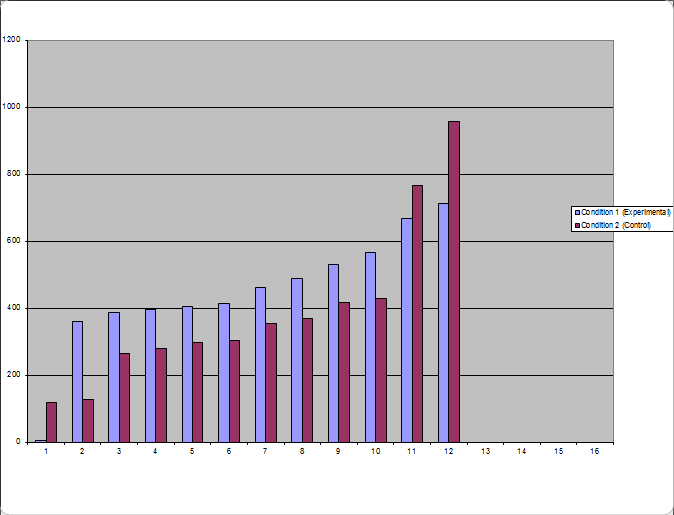
\includegraphics[width=\textwidth]{table1}
\subsection{Comparison of mean values of given groups}
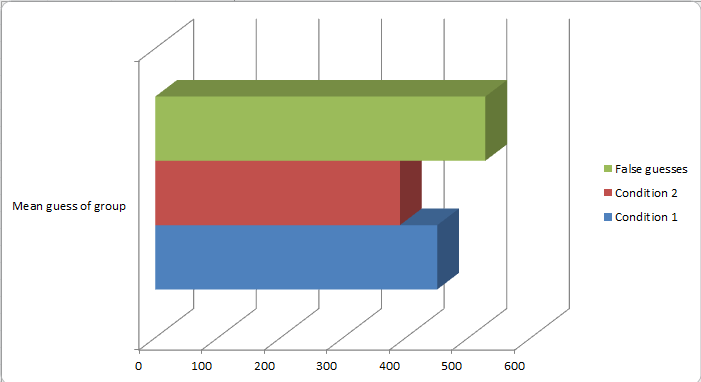
\includegraphics[width=\textwidth]{table2}
\subsection{Range of given groups values}
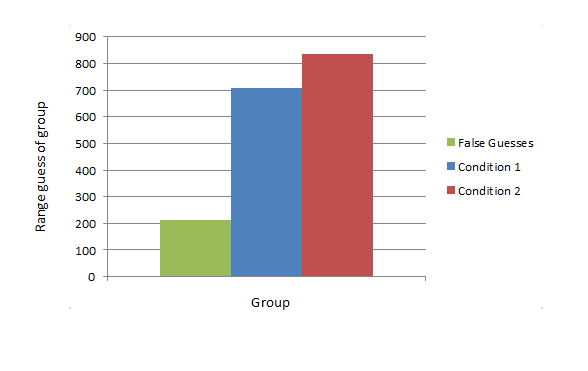
\includegraphics[width=\textwidth]{table3}

\section{Discussion}
The results shown highlight that the experimental group (condition 1) had an average answer closer to the previous guesses than the control (condition 2). This suggests that the individuals conformed to the previous guesses, despite the influencing majority being unseen. The lower range in condition 1 than condition 2 also supports the hypothesis as it shows that the individuals in condition 1 were more consistent with their answers, as they had the answers of the false guesses for guidance. Some confounding variables may have been identified; one of these is the fact that one individual guessed 5 in condition 1 (see Appendix C - Raw data table). This has been identified as a statistical anomaly or outlier. This individual either did not fully understand the task at hand or they were not taking the experiment seriously. This did not sway the results enough to change the overall conclusions drawn from the data however, so the experiment needn’t be done again. Another confounding variable identified is that the individuals may have been pressured by the situations and may have not answered in their “true answer.” This is a potential weakness of the study, as it means that individuals are not answering naturally in an ecologically valid environment. The results shown in Study of Informational Conformity with an unknown majority (2018) show an example of informational influence as only the results of the falsified previous guesses were present. There were no physical bodies there to inflict normative influence. The individuals in this study were purely influenced by the information of the “previous answers” alone. The individuals in this study believed the previous answers to be a guidance point for them. The results found in this study relate to the factor affecting conformity of group size. The optimal group size for conformity was found by Asch (1956)1 to be between 3 and 7. This study operates on this optimal level as there was 6 previous guesses on the falsified guess sheets, therefore increasing potential conformity. This study also connects with the work of Asch (1951) as it is again a study which shows individuals conforming to a majority on a given task. The 2018 study differs from Asch’s landmark study in that in this study, the majority was not seen. This study also connects to Jenness (1932) In that it involved individuals making a judgement in an ambiguous task, with the hope that the individual will be affected by informational conformity and will look to the others for guidance on their answer. The findings of the study can suggest many real world applications such as explaining how social media can influence people into changing their opinions. While they cannot directly see these people, they still influence people. The results found suggest that people can be influenced by an unseen majority, meaning that we could be influenced by artificial majorities in the real world; a group could lie about their number of supporters to influence others to conform.  This research could be taken further in the same field by seeing whether or not previous fake “voice cues” will affect conformity further than pure text cues. The conclusions drawn from this study are that an individual will conform to a majority when making a judgement on an uncertain task, even when the majority is unknown and unseen.
\appendix
\appendixpage
\addappheadtotoc
\chapter{Guess sheets with previous falsified guesses}
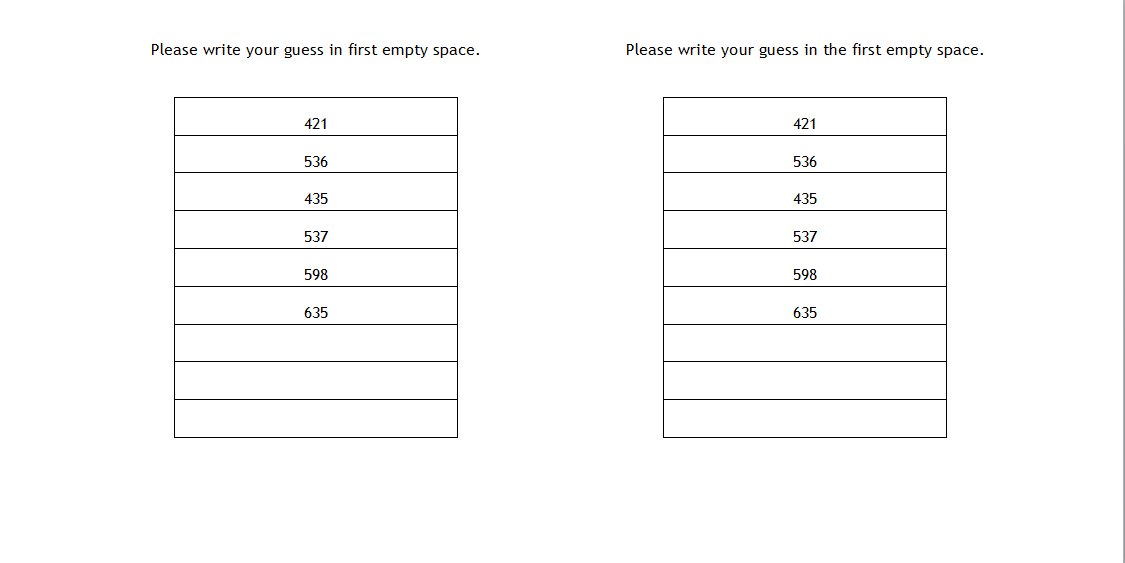
\includegraphics[width=\textwidth]{psych1}
\chapter{Blank guess sheets}
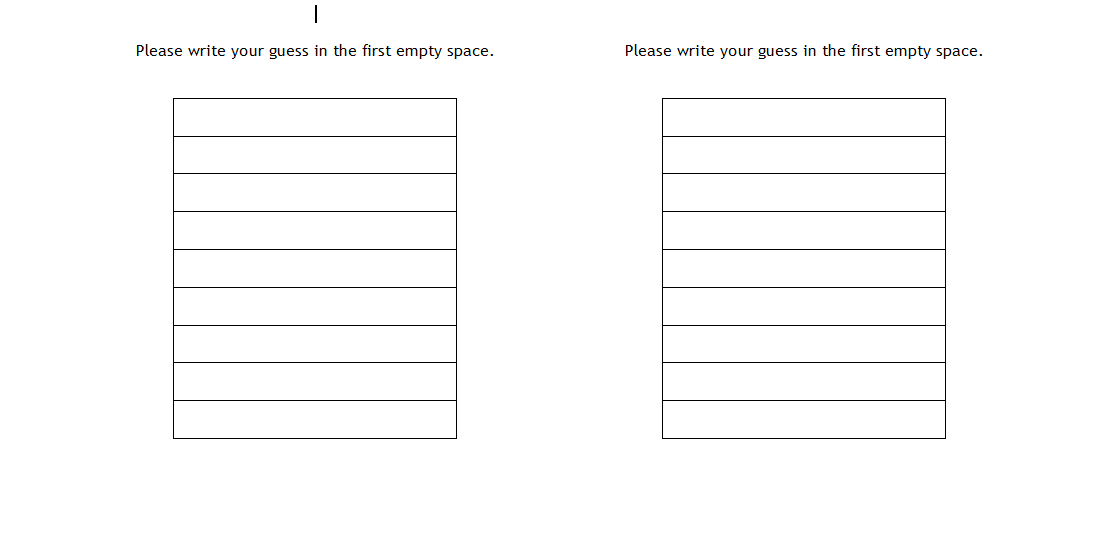
\includegraphics[width=\textwidth]{psych2}
\chapter{Raw results table}
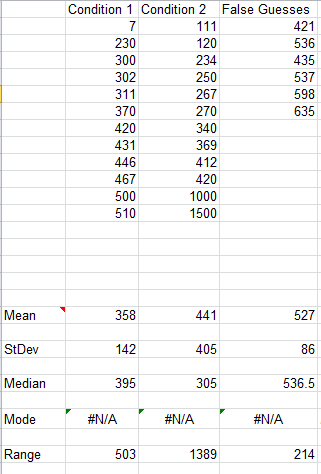
\includegraphics[width=\textwidth]{psych3}
\chapter{Informed consent document}
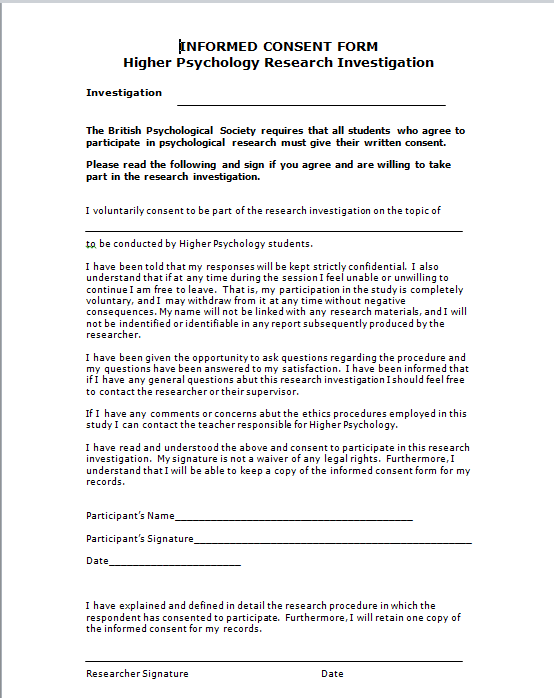
\includegraphics[width=\textwidth]{psych4}
\chapter{Information sheet for participants}
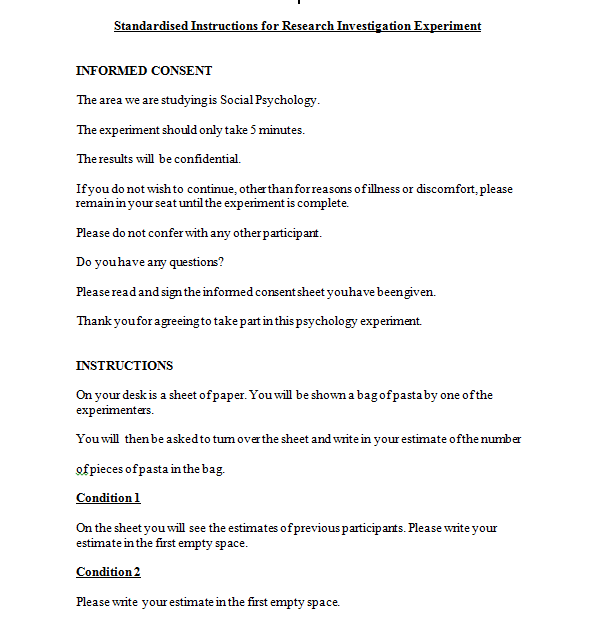
\includegraphics[width=\textwidth]{psych5}
\end{document}
